\def\currentRootFolder{chapter/modelOfIntegratedRate/neutrinoMassMeasurement}
\def\currentFigureFolder{\currentRootFolder/fig}
\newcommand{\elecIndex}{\mathrm{e}}

\newcommand{\Bsource}{B^j_\mathrm{S}}
\newcommand{\BsourceAvg}{B_\mathrm{S}}
\newcommand{\zSource}{z_\mathrm{S}}
\newcommand{\thetaSource}{\theta_\mathrm{S}}
\newcommand{\thetaSourceAvg}{\theta_\mathrm{S}}
\newcommand{\Esource}{E_\mathrm{S}}
\newcommand{\Usource}{U^j_\mathrm{S}}
\newcommand{\gammaSource}{\gamma_\mathrm{S}}


\newcommand{\Bps}{B_\mathrm{PS2}}
\newcommand{\Bana}{B_\mathrm{A}}
\newcommand{\Bpinch}{B_\mathrm{P}}
\newcommand{\Bmax}{B_\mathrm{max}}
\newcommand{\Bmin}{B_\mathrm{min}}

\newcommand{\thetaMax}{\theta_\mathrm{max}}
\newcommand{\Esur}{E_\mathrm{sur}}
\newcommand{\detEff}{\epsilon_\mathrm{det}}
\newcommand{\macefilterwidth}{\Delta \mathcal{E}^j(\thetaS^j)}

\newcommand{\EtransPure}{E^j_\mathrm{tr}}
\newcommand{\Etrans}{\EtransPure(qU,\Esource,\thetaSource)}
\newcommand{\thetaTransPure}{\theta^j_\mathrm{tr}}
\newcommand{\thetaTrans}{\thetaTransPure(\Esource,qU)}

\newcommand{\As}{A_\mathrm{S}}
\newcommand{\Rbg}{R_\mathrm{bg}}


\newacronym{standardmodel}{SM}{Standard Model of Particle Physics}
\newacronym{lep}{LEP}{Large Electron Positron Collider}
\newacronym{ssm}{SSM}{standard solar model}

\section{A KATRIN Neutrino Mass Measurement}
\label{sec:katrinExpNuMassMeasurement}
\begin{figure}
	\centering
	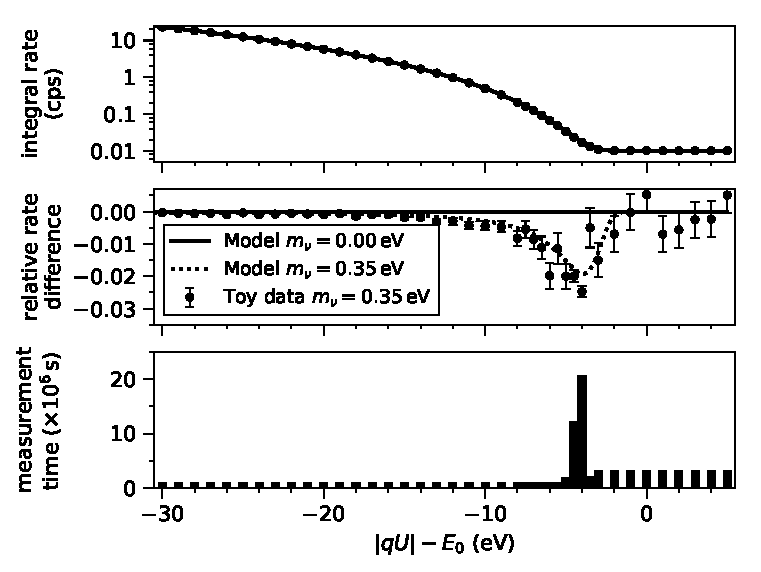
\includegraphics[width=\textwidth]{\currentFigureFolder/neutrinoMassMeasurement.pdf}
	\xcaption{Simulated KATRIN measurement for a non-vanishing neutrino mass.}{Simulated KATRIN measurement for a non-vanishing neutrino mass.}{The top plot shows the measured integrated rate $\Gamma$ in dependence of the retarding energy. The plot in the middle shows the relative rate difference for a non-vanishing neutrino mass $\Gamma(\nuMass=\SI{0.35}{eV})/\Gamma(\nuMass=\SI{0}{eV})-1$. The difference is $\sim\SI{2}{\percent}$ at a retarding energy approximately $\SI{4}{eV}$ below the endpoint. The bottom plot shows the \gls{mtd} where most measurement time is attributed to the most sensitive region. This is also visible in the size of the uncertainty bars of the toy data.}
	\label{fig:katrinExpNuMassMeasurement}
\end{figure}


\todo{Introduction, Clean up and cite/refer equation}
The predicted counts for a retarding energy of $qU$ when measuring a duration $t(qU)$ are
\begin{equation}
\label{eq:intSpecModelCountsFinal}
\bar{N}(qU) = t(qU) \cdot \detEff \cdot \left(
\As \cdot
\sum_{j}
N_T^j \cdot
\int_{qU}^{E_0} 
\left(\frac{\d \Gamma(\Esource)}{ \d \Esource}\right) \cdot 
\bar{R}^j(\Esource, qU) 
\d \Esource +
\Rbg
\right)
\fullstop
\end{equation}
Here, $\As=1$ is a normalization factor, $\detEff \in [0,1]$ is the detector efficiency \todo{reference KATRIN chapter}, the sum goes over all source slices with label $j$, $N_T^j$ is the number of tritium molecules in the $j$th source slice, $\left(\d \Gamma(\Esource) / \d \Esource \right)$ is the differential rate from \eqref{eq:intSpecModelDiffSpec}, $\bar{R}^j(\Esource, qU)$ is the response function from \eqref{eq:} and $\Rbg$ is the rate of background events.

KATRIN measures electron counts as described in equation \eqref{eq:intSpecModelCountsFinal} at a set of retarding energies $\left\{qU_i\right\}$. How much measurement time $t(qU_i)$ is attributed to a certain retarding energy is called a \glsentryfull{mtd}. The \gls{mtd} influences the experiment's sensitivity to the neutrino mass. An optimal \gls{mtd} balances the following aspects~\cite{Angrik:2005ep}:
\begin{enumerate}
	\item Some measurement time has to be attributed to retarding energies beyond the endpoint of the spectrum to determine the background rate. The optimal duration depends on the background rate.
	\item The shape of the integral tritium $\upbeta$ spectrum depends the strongest on the neutrino mass near its endpoint $E_0$ \eqref{eq:intSpecModelEndpoint}.
	\item Measurements deeper into the spectrum increase the count rate and hence, lower the statistical uncertainty due to Poisson statistics. They mainly determine the endpoint from extrapolating the $\upbeta$ spectrum.
	\item The theoretical description of the integral tritium-$\upbeta$ spectrum is optimized for the endpoint region. E.\,g.~the molecular final states (Rydberg states and the electronic continuum) for $\upbeta$-electron energies \SI{40}{eV} below the endpoint would need further investigation~\cite{Doss:2006}. Hence, deeper scans introduce modeling uncertainties. However, it is expected that continuous modeling efforts decrease these uncertainties.
\end{enumerate}
The KATRIN Design Report \cite{Angrik:2005ep} suggests 5 \gls{mtd}s for different measurement ranges $[E_0-\alpha\;\SI{}{eV}, E_0 + \SI{5}{eV}]$ with $\alpha \in \{20, 25, 30, 40, 50\}$ and the conclusion that $\alpha=30$ yields the best sensitivity to the neutrino mass. Figure~\ref{fig:katrinExpNuMassMeasurement} shows a KATRIN measurement for the \SI{30}{eV} range and a total measurement time of three years. The distortion of the measured integrated rate by a non-vanishing neutrino mass can be seen approximately \SI{-4}{eV} below the endpoint.

Depending 
Furthermore, searches for sterile neutrinos at the keV-scale would require deeper scans~\cite{Kleesiek2014}. Several measurement campaigns were already conducted. The \gls{ft} commissioning campaign successfully proved the apparatus functioning. The corresponding \gls{mtd} covered a range starting at $\sim E_0-\SI{1.6}{keV}$. The \gls{knm1} campaign is evaluated during the writing of this thesis. It set out to establish an unprecedented limit on the neutrino mass by $\upbeta$-decay measurements. Its \gls{mtd} starts at $\sim E_0-\SI{90}{eV}$.